\section{The Proposed Method -Blood Smears object detection using DCGAN network}
\label{segmethod}

In this section, We describe a process for object detection in malaria blood smears using GAN networks. The process consist of the following  steps: blood smears image acquisition, image generation with GANs networks (Figure \ref{fig:maincomp} -\ding{202} ); train a convolutional neural network (Figure \ref{fig:maincomp} -\ding{203});  apply adaptive  threshold filter (Figure \ref{fig:maincomp} -\ding{204}) and classify objects with the trained convolutional network (Figure \ref{fig:maincomp} -\ding{205}). 

\begin{figure*}[h]
\caption{Process for object detection in malaria blood smears using DCGAN networks}
\label{fig:maincomp}
  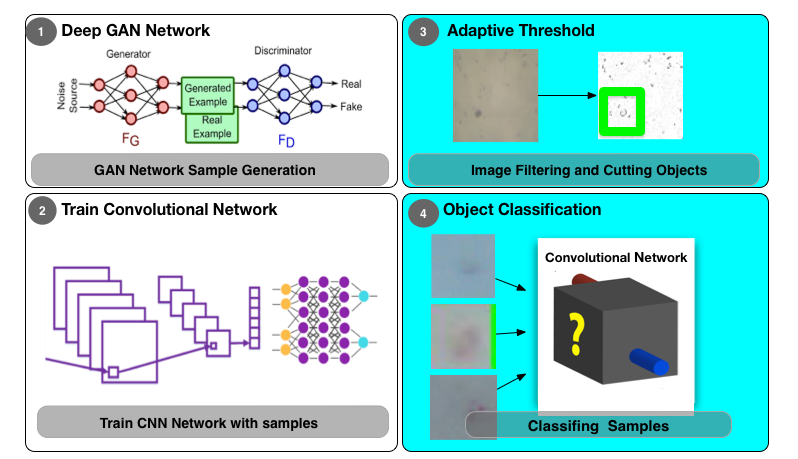
\includegraphics[width=\textwidth]{images/MainComponents.png}
\end{figure*}

Several experiments where conducted in order to analyze the benefits of use GAN networks in the proposed method. The real blood smears images for the experiments where acquired from the repository presented by Quinn et al. \cite{Quinn2016DeepDiagnostics}.  The code are developed in python language using the Keras framework.

\subsection{DCGAN Network Sample Generation}

The experiments used a Deep convolutional generative adversarial network (DCGAN) proposed by Radford et al. \cite{Radford2015}, according to the code as shown in listing \ref{lst:gen} and \ref{lst:dis}. The Generator receive as input a noise vector (Listing \ref{lst:gen}- lines 3 and 4) which passes through convolutional, normalization , upsampling and activation layers. Batch Normalization normalizing activations throughout the network, it prevents small changes to the parameters from amplifying into larger and suboptimal changes in activations in gradients; for instance, it prevents the training from getting stuck in the saturated regimes of nonlinearities. The Relu activation is used in the generator with the exception of the output layer which uses the Tanh function. DCGAN  was trained with 1800 real plasmodium images cutted from real blood smears images.




\lstset{basicstyle=\footnotesize\ttfamily,breaklines=true}
\begin{lstlisting}[language=Python,numbers=left,frame=tb,caption=Generator Keras Code]
model = Sequential()

model.add(Dense(512 * 7* 7, activation="relu",     
input_dim=self.latent_dim))

model.add(Reshape((7,7, 512)))
model.add(UpSampling2D())
model.add(Conv2D(256, kernel_size=3, padding="same"))
model.add(BatchNormalization(momentum=0.8))
model.add(Activation("relu"))
model.add(UpSampling2D())
model.add(Conv2D(128, kernel_size=3, padding="same"))
model.add(BatchNormalization(momentum=0.8))
model.add(Activation("relu"))
model.add(UpSampling2D())
model.add(Conv2D(64, kernel_size=3, padding="same"))
model.add(BatchNormalization(momentum=0.8))
model.add(Activation("relu"))
model.add(UpSampling2D())
model.add(Conv2D(32, kernel_size=3, padding="same"))
model.add(BatchNormalization(momentum=0.8))
model.add(Activation("relu"))
model.add(Conv2D(self.channels, 
            kernel_size=3, padding="same"))
model.add(Activation("tanh"))

model.summary()

noise = Input(shape=(self.latent_dim,))
img = model(noise)

\end{lstlisting}


\lstset{basicstyle=\footnotesize\ttfamily,breaklines=true}
\begin{lstlisting}[language=Python,numbers=left,frame=tb,caption=Discriminator source code,label=lst:dis,xleftmargin=2em]
model = Sequential()

model.add(Conv2D(8, kernel_size=3, strides=2, input_shape=self.img_shape, padding="same"))
model.add(LeakyReLU(alpha=0.2))
model.add(Dropout(0.25))
model.add(Conv2D(16, kernel_size=3, strides=2, padding="same"))
        
model.add(BatchNormalization(momentum=0.8))
model.add(LeakyReLU(alpha=0.2))
model.add(Dropout(0.25))
model.add(Conv2D(32, kernel_size=3, strides=2, padding="same"))
model.add(BatchNormalization(momentum=0.8))
model.add(LeakyReLU(alpha=0.2))
model.add(Dropout(0.25))
model.add(Conv2D(64, kernel_size=3, strides=2, padding="same"))
model.add(BatchNormalization(momentum=0.8))
model.add(LeakyReLU(alpha=0.2))
model.add(Dropout(0.25))
model.add(Conv2D(128, kernel_size=3, strides=2, padding="same"))
model.add(BatchNormalization(momentum=0.8))
model.add(LeakyReLU(alpha=0.2))
model.add(Dropout(0.25))
model.add(Conv2D(256, kernel_size=3, strides=1, padding="same"))
model.add(BatchNormalization(momentum=0.8))
model.add(LeakyReLU(alpha=0.2))
model.add(Dropout(0.25))

model.add(Flatten())
model.add(Dense(1, activation='sigmoid'))

model.summary()

img = Input(shape=self.img_shape)
validity = model(img)

\end{lstlisting}

Figs. \ref{fig:gen50},\ref{fig:gen250} and \ref{fig:gen30410} presents the images generated after 50,250 and 30410 epochs.


\begin{figure}[h]
\caption{Generated images after 50 epochs}
\label{fig:gen50}
\begin{center}
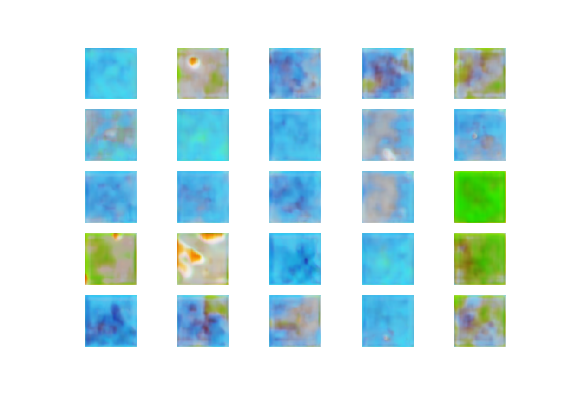
\includegraphics[scale=0.45]{./images/generation/alta_mnist_50.png} \end{center}
\end{figure}

\begin{figure}[h]
\caption{Generated images after 250 epochs}
\label{fig:gen250}
\begin{center}
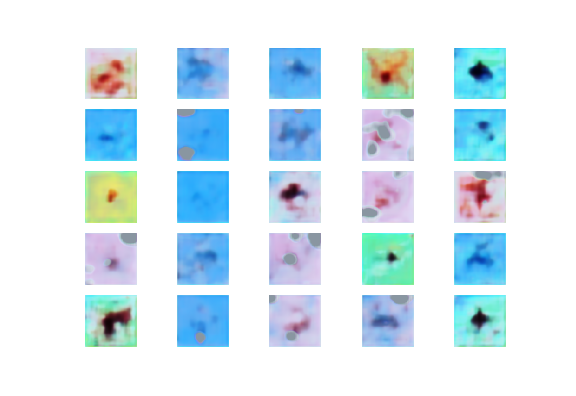
\includegraphics[scale=0.45]{./images/generation/alta_mnist_250.png} \end{center}
\end{figure}

\begin{figure}[h]
\caption{Generated images after 30410 epochs}
\label{fig:gen30410}
\begin{center}
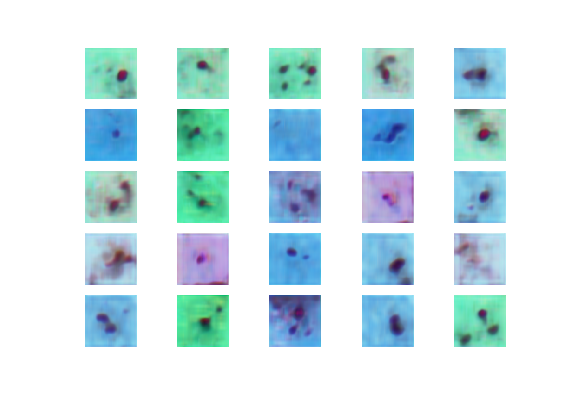
\includegraphics[scale=0.45]{./images/generation/alta_mnist_30410.png} \end{center}
\end{figure}

\subsection{Train CNN network with samples}



After the generation of the images by the DCGAN network, We use  data augmentation techniques to train a CNN . We follow the simple data augmentation for training: pixels are padded on each side, and a 50x50 crop is randomly sampled from the padded image or its horizontal flip.  This allows the network to learn invariance to deformations. Data augmentation is essential to teach the network the desired invariance and robustness properties, when only few training samples are available and realistic deformations can be simulated efficiently.


\begin{figure*}[htp]
  \label{fig:threshold}
  \centering
  \subfigure[Blood smears image with Adaptive Thresholding]{
  %\caption{Generated images after 30410 epochs}
  %\label{fig:threshold}
  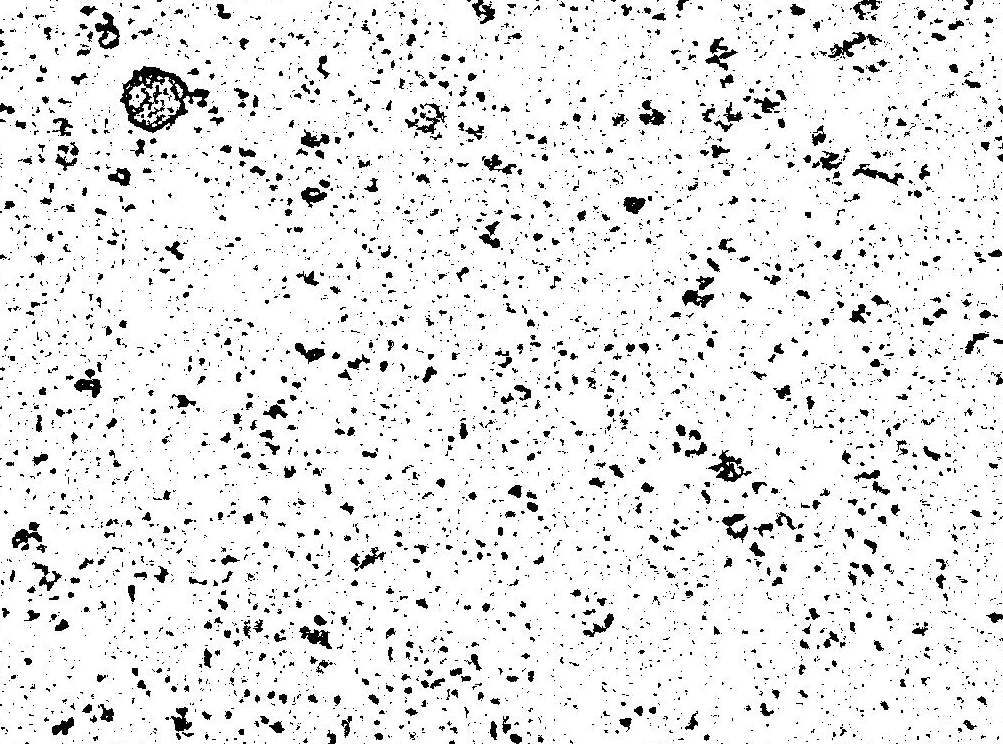
\includegraphics[scale=0.21]{./images/threshold.png}
  }
  \subfigure[Blood smears image with object detection]{
  %\caption{Generated images after 30410 epochs}
  %\label{fig:objectdetect}
  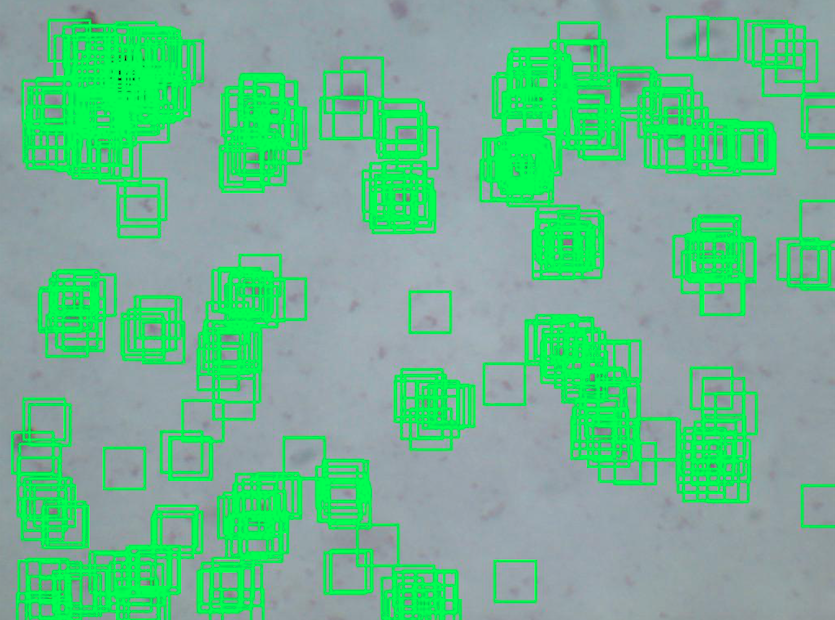
\includegraphics[scale=0.25]{./images/object_detected.png}
  }
\end{figure*}

The images are used to train a CNN network. Table \ref{tab:results} presents the results for eight executions. The CNN network was trained with generated images and tested with real images. With 2200 generated images by the DCGAN network, the CNN network obtain 100\% of accuracy with the real images. From the results presented in the experiments, we observe that the images generated by the DCGAN network can be used in the training of a CNN network to detect objects improving classifier accuracy.

% Please add the following required packages to your document preamble:
% \usepackage[table,xcdraw]{xcolor}
% If you use beamer only pass "xcolor=table" option, i.e. \documentclass[xcolor=table]{beamer}
\begin{table}[h]
\caption{Results of training the CNN network with images generates by DGAN network}
\label{tab:results}
\begin{tabular}{|l|l|l|l|}
\hline
\rowcolor[HTML]{C0C0C0} 
\textbf{\begin{tabular}[c]{@{}l@{}}Number of \\ Samples \\ Created\\ by GAN \\ Network\end{tabular}} & \textbf{\begin{tabular}[c]{@{}l@{}}Number of\\ Real \\ Images\\ for Test\end{tabular}} & \textbf{\begin{tabular}[c]{@{}l@{}}Number \\ of correctly \\ classified \\ samples\end{tabular}} & \textbf{\begin{tabular}[c]{@{}l@{}}Number of \\ incorrectly \\ classified \\ samples\end{tabular}} \\ \hline
600                                                                                            & 600                                                                                 & 420 (70 \%)                                                                                      & 180                                                                                                \\ \hline
800                                                                                            & 600                                                                                 & 406 (68 \%)                                                                                      & 194                                                                                                \\ \hline
1000                                                                                           & 600                                                                                 & 453 (76 \%)                                                                                      & 147                                                                                                \\ \hline
1200                                                                                           & 600                                                                                 & 424 (71 \%)                                                                                      & 176                                                                                                \\ \hline
1400                                                                                           & 600                                                                                 & \begin{tabular}[c]{@{}l@{}}429 \\ ($\sim$71 \%)\end{tabular}                                     & 171                                                                                                \\ \hline
1600                                                                                           & 600                                                                                 & 430 (72 \%)                                                                                      & 170                                                                                                \\ \hline
1800                                                                                           & 600                                                                                 & 480 (80  \%)                                                                                     & 120                                                                                                \\ \hline
2200                                                                                           & 600                                                                                 & 600 (100 \%)                                                                                     & 0                                                                                                  \\ \hline
\end{tabular}
\end{table}

\subsection{Image Filtering and Cutting Objects}

We use an adaptive threshold filter in the the blood smear images.  Thresholding is a method of image segmentation where each pixel in an image with a black pixel if the image intensity ${\displaystyle I_{i,j}} I_{{i,j}}$ is less than some fixed constant T (that is, ${\displaystyle I_{i,j}<T} I_{{i,j}}<T)$, or a white pixel if the image intensity is greater than that constant. Adaptive Thresholding is a form of extract useful information encoded into pixels while minimizing background noise. We use OpenCV to find the contours and centers of objects.

\subsection{Classifying Samples with CNN network}

Finally,  with center of all objects, image segments where cutted from the blood smears image and classified by the CNN network. Fig. \ref{fig:threshold} - (b) present a sample of objects detected by the proposed process.